\section{NET\_10 --- VXLAN and Ethernet VPNs}


\subsection{Datacenter Networks}

Le reti di \emph{data center} si distinguono da quelle tipiche degli ISP perché sono progettate principalmente per sostenere traffico \emph{est-ovest} (server--server) su larga scala, con requisiti stringenti di scalabilità, isolamento e continuità di servizio. Per gestire migliaia di host mantenendo prestazioni prevedibili, si adottano architetture a più livelli (tier) e, nelle soluzioni moderne, si separano spesso \emph{underlay} (rete IP instradata) e \emph{overlay} (virtualizzazione e segmentazione per tenant).


\subsubsection{Basic Tree Datacenter Networks}

\begin{figure}[H]
\centering
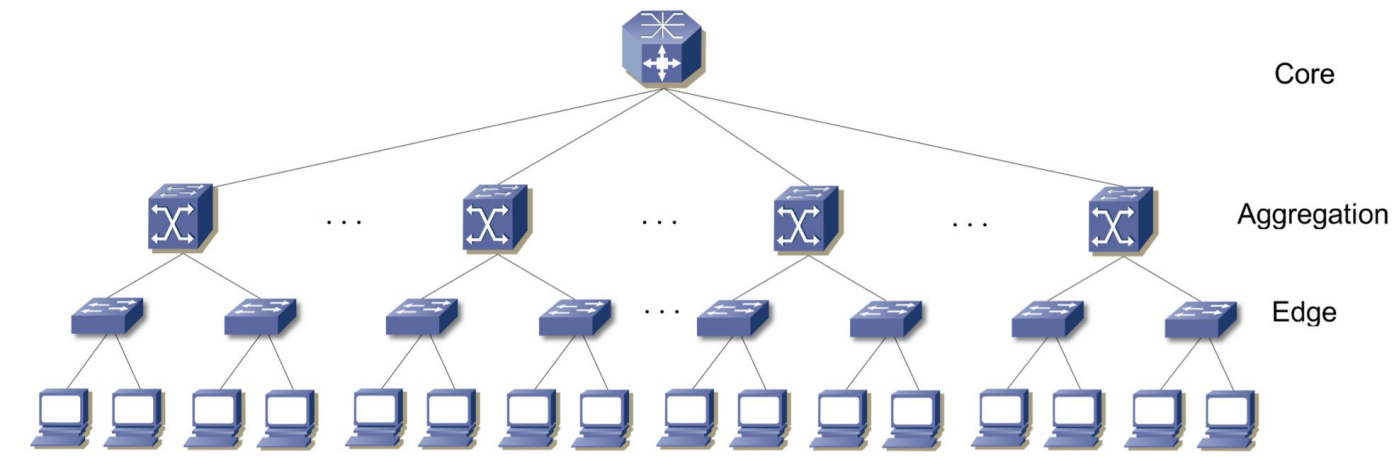
\includegraphics[width=0.78\textwidth]{immagini/NET_10/basic_tree_topology.png}
\caption{Topologia \emph{basic tree} in un data center: i server sono aggregati su switch di \emph{edge/access}, poi su \emph{aggregation} e infine sul \emph{core}.}
\label{fig:net10-basic-tree}
\end{figure}


\paragraph{Basic Tree tiers: Access/ToR, Aggregation/EoR, Core switches}

Una prima architettura “classica” è la topologia ad albero (\emph{basic tree}), organizzata in tre tier:

\emph{Access/ToR} (Top-of-Rack), \emph{Aggregation/EoR} (End-of-Rack) e \emph{Core}.
\begin{figure}[H]
\centering
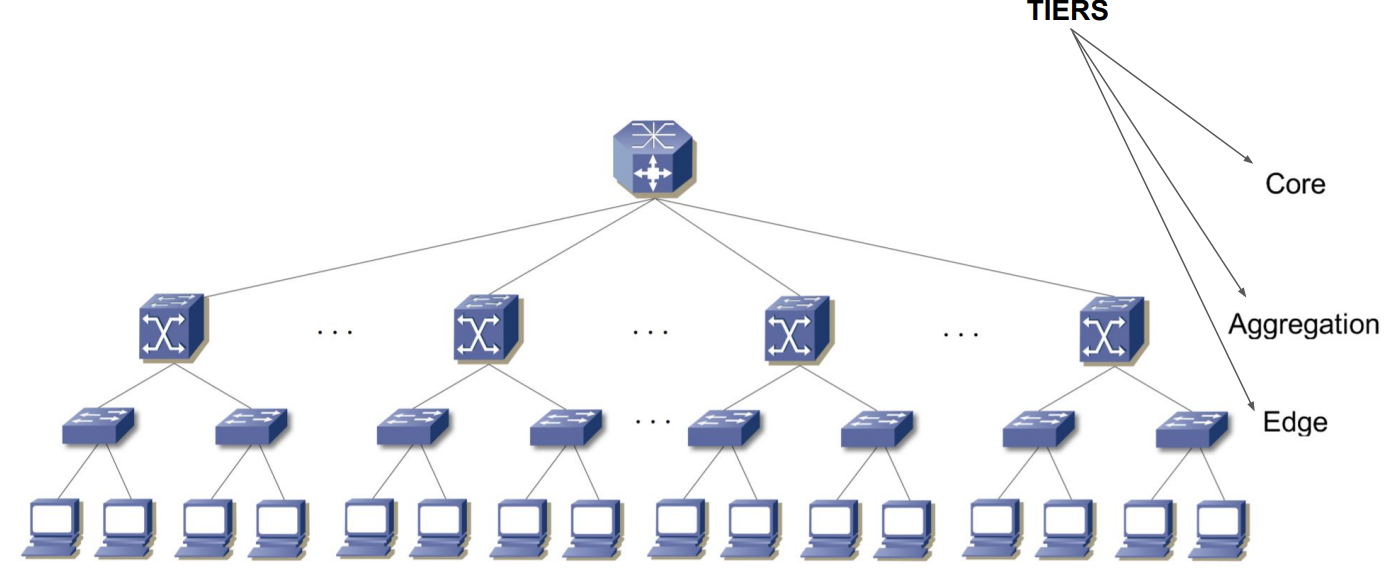
\includegraphics[width=0.78\textwidth]{immagini/NET_10/basic_tree_tiers.png}
\caption{Suddivisione a tre livelli della topologia \emph{basic tree}: \emph{edge/access} (ToR), \emph{aggregation} (EoR) e \emph{core}.}
\label{fig:net10-basic-tree-tiers}
\end{figure}


I ToR costituiscono il livello più basso: sono gli switch posizionati tipicamente in cima al rack e aggregano le connessioni dei server, fornendo l’accesso alla rete del data center. Gli switch di aggregazione (EoR) raccolgono il traffico di più ToR, riducendo il numero di collegamenti verso l’alto e concentrando i flussi. Infine, i core switch rappresentano il “cuore” della rete: gestiscono il traffico complessivo, devono sostenere banda aggregata elevata e, nella pratica, includono spesso anche la connettività verso l’esterno (uplink verso Internet o verso reti WAN/enterprise).


\paragraph{Basic Tree: limitations}

Questa architettura presenta due limiti strutturali. Il primo è l’\emph{oversubscription} sul core: i core switch devono sostenere (nel caso peggiore) l’intera banda aggregata proveniente dai tier inferiori, rendendo complesso (e costoso) dimensionare correttamente la rete all’aumentare degli host. Il secondo è la \emph{scarsa fault tolerance}: un guasto su un nodo di livello alto o su collegamenti critici può isolare interi “rami” dell’albero, con impatto diretto sulla disponibilità. A ciò si aggiunge il fatto che gli switch dei tier superiori tendono a essere dispositivi più costosi proprio perché devono supportare throughput e capacità maggiori.


\subsubsection{Clos-based Datacenter Networks}


\paragraph{Today’s Data Center networks: key objectives}

Le reti di data center moderne sono progettate attorno a obiettivi operativi chiari: (i) \emph{scalabilità}, per espandere progressivamente compute e rete senza riprogettare l’architettura; (ii) \emph{ridondanza}, evitando single point of failure a più livelli; (iii) \emph{latenza} contenuta e soprattutto prevedibile, riducendo il numero di hop; (iv) \emph{capacità di rete} elevata, per sostenere applicazioni distribuite e traffico est-ovest; (v) \emph{tenant isolation}, necessario nei contesti cloud per separare traffico e performance tra clienti diversi anche su infrastruttura condivisa.


\paragraph{Clos two-tier: leaf-spine topology}

Per soddisfare questi requisiti, l’architettura di riferimento è la \emph{Clos topology}. Nel caso più comune a due tier (\emph{leaf-spine}), gli switch \emph{leaf} connettono i server (o i rack) e sono connessi in modo ridondante a tutti gli switch \emph{spine}. Il risultato è una fabric con molti percorsi equivalenti tra qualunque coppia di leaf: la rete è “piatta” rispetto al forwarding, riduce i colli di bottiglia tipici dei tree e abilita un bilanciamento del traffico più efficace.

\begin{figure}[H]
\centering
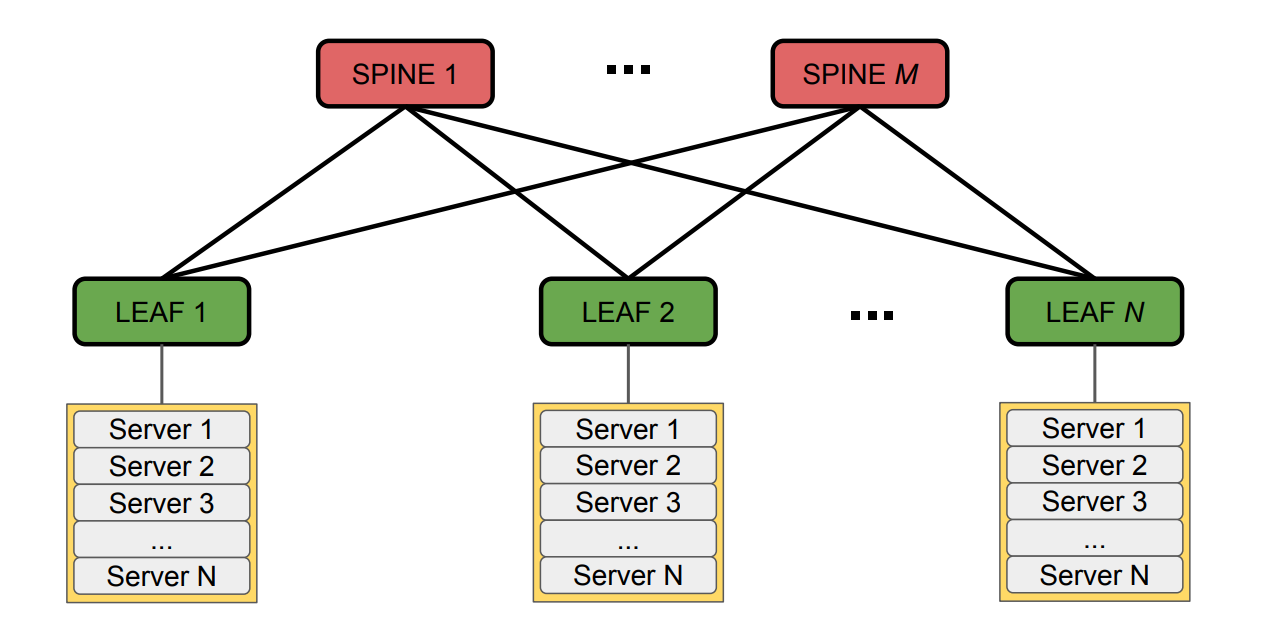
\includegraphics[width=0.82\textwidth]{immagini/NET_10/leaf_spine_topology.png}
\caption{Topologia \emph{leaf-spine}: ogni leaf è connessa in modo ridondante a tutte le spine, ottenendo molti cammini equivalenti tra qualsiasi coppia di leaf.}
\label{fig:net10-leaf-spine}
\end{figure}


\paragraph{Scalability: need more bandwidth and compute capacity}

La scalabilità in una leaf-spine è \emph{incrementale}:

se serve più banda complessiva, si può aggiungere una nuova \emph{spine} e collegarla a tutte le leaf, aumentando il numero di percorsi e la capacità di bisezione. Se invece serve aumentare la capacità computazionale (nuovi rack/server), si aggiunge una nuova \emph{leaf} e la si collega a tutte le spine esistenti, integrando nuovi end-host senza cambiare il disegno di base della rete.
\begin{figure}[H]
\centering
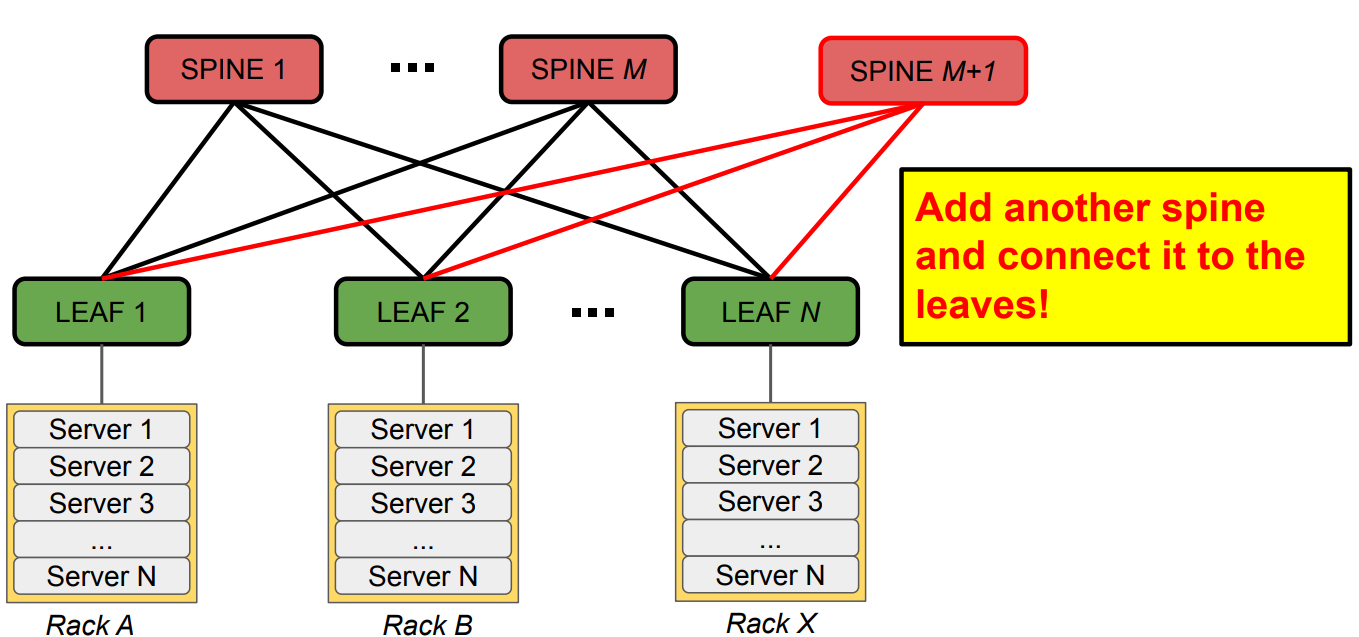
\includegraphics[width=0.5\textwidth]{immagini/NET_10/scale_add_spine.png}
\caption{Scalabilità in leaf-spine: per aumentare la capacità complessiva della fabric si aggiunge una nuova \emph{spine} e la si collega a tutte le leaf.}
\label{fig:net10-scale-add-spine}
\end{figure}

\begin{figure}[H]
\centering
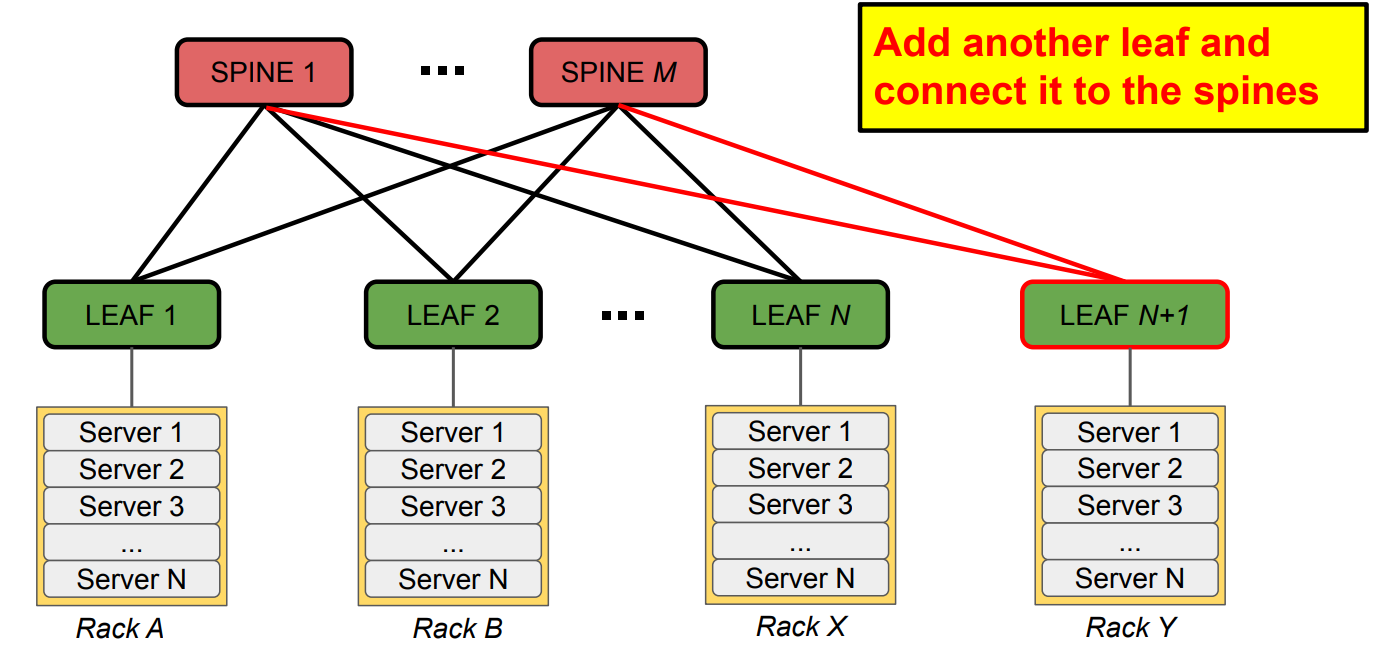
\includegraphics[width=0.5\textwidth]{immagini/NET_10/scale_add_leaf.png}
\caption{Scalabilità in leaf-spine: per aumentare la capacità di calcolo (nuovi rack/server) si aggiunge una nuova \emph{leaf} collegandola a tutte le spine esistenti.}
\label{fig:net10-scale-add-leaf}
\end{figure}


\paragraph{Fault tolerance: Spines}

La ridondanza dello strato spine migliora la resilienza: se una spine si guasta (o viene tolta per manutenzione), la raggiungibilità tra leaf resta garantita tramite le spine rimanenti. Inoltre, con un underlay instradato, i protocolli di routing possono rilevare fault di link/nodi e riconvergere, riallocando i flussi su percorsi alternativi.

\begin{figure}[H]
\centering
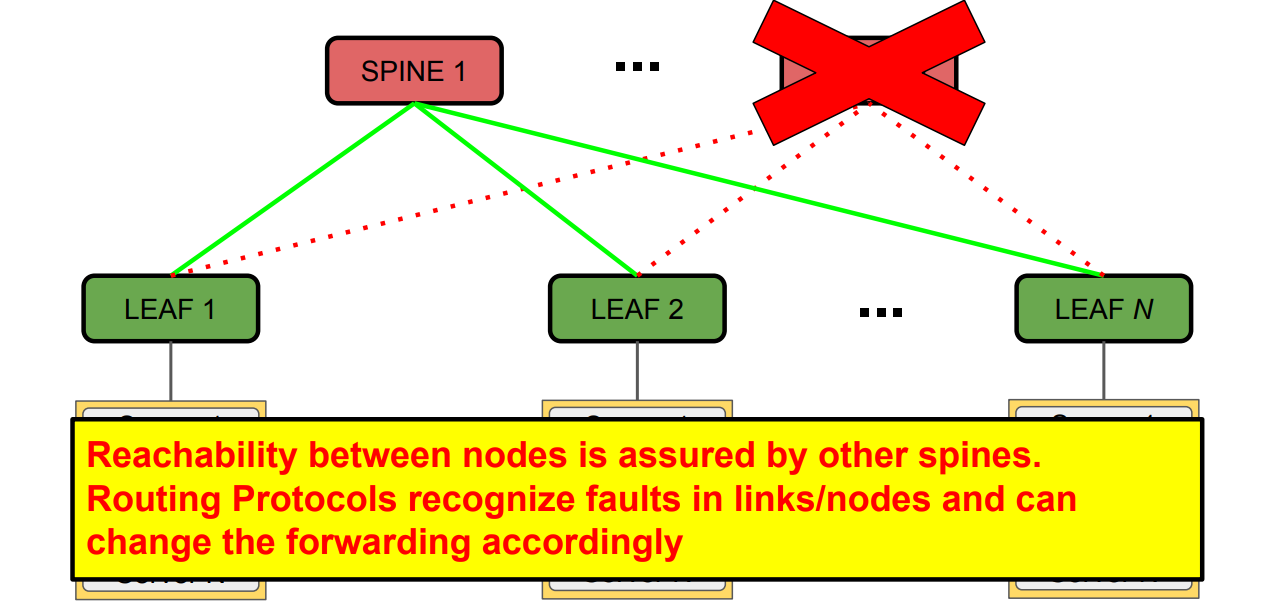
\includegraphics[width=0.82\textwidth]{immagini/NET_10/fault_spines.png}
\caption{Fault tolerance nello strato spine: la perdita di una spine mantiene la raggiungibilità grazie ai cammini alternativi sulle spine rimanenti.}
\label{fig:net10-fault-spines}
\end{figure}
\paragraph{Fault tolerance: Leaves}

La leaf è un punto di aggregazione “vicino” ai server: se una leaf singola fallisce, i rack/host collegati a quella leaf possono perdere connettività. Per mitigare questo rischio, si ricorre a meccanismi di multi-homing (dual attachment) dei server verso coppie di leaf, così che la perdita di uno switch non interrompa il servizio.
\begin{figure}[H]
\centering
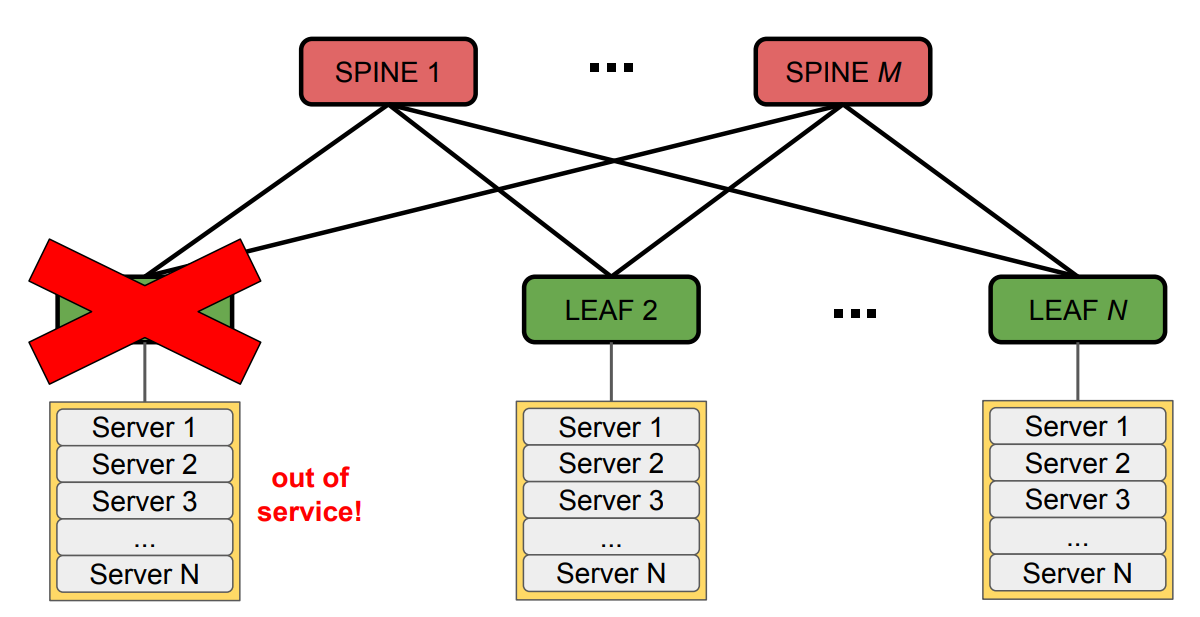
\includegraphics[width=0.82\textwidth]{immagini/NET_10/fault_leaves.png}
\caption{Fault tolerance lato leaf: un guasto di una leaf può isolare i server collegati a quello switch, motivo per cui si usa spesso multi-homing verso coppie di leaf.}
\label{fig:net10-fault-leaves}
\end{figure}

\paragraph{Fault tolerance: LAG and MLAG}

Due tecniche comuni per rendere robusto l’accesso sono:

\emph{LAG} e \emph{MLAG}. Il \emph{Link Aggregation Group} aggrega più link fisici in un unico link logico, ottenendo sia aumento di banda (somma delle capacità) sia ridondanza (se un link fisico cade, il canale logico resta attivo). Il \emph{Multi-Chassis LAG} estende il concetto su due switch distinti: lato server si presenta un’unica aggregazione logica, ma i link terminano su due leaf diverse, aggiungendo ridondanza anche a livello di switch (non solo di singolo collegamento).
\begin{figure}[H]
\centering
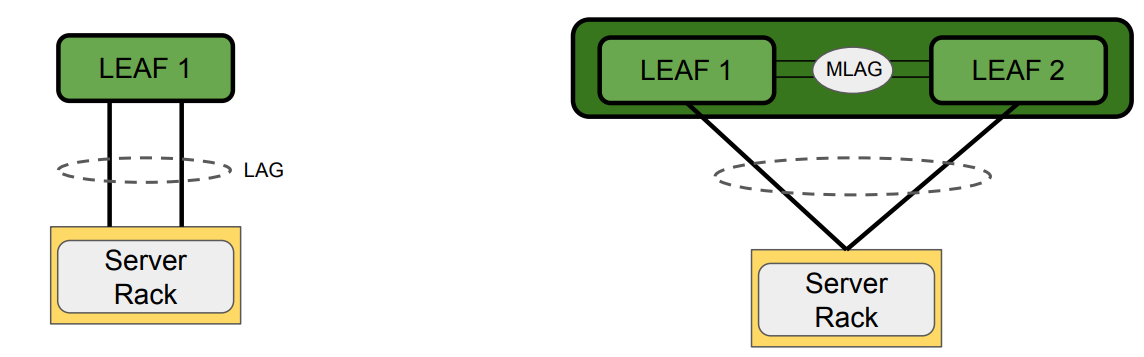
\includegraphics[width=0.72\textwidth]{immagini/NET_10/lag_mlag.png}
\caption{LAG e MLAG: l’aggregazione di link aumenta banda e ridondanza; MLAG estende la ridondanza anche al livello di switch (terminazioni su due leaf diverse).}
\label{fig:net10-lag-mlag}
\end{figure}

\paragraph{Latency}

In un data center la latenza dipende soprattutto dal numero di hop, dato che il tempo di trasmissione “sul filo” è spesso trascurabile rispetto a elaborazione e attraversamenti. Si introduce quindi il concetto di \emph{network diameter} (massimo numero di hop tra due nodi lungo i cammini minimi). Nelle leaf-spine, il diametro tra end-host in rack diversi è tipicamente costante e basso (in molti casi 2 hop leaf→spine→leaf), rendendo la latenza più prevedibile.


\paragraph{Bandwidth and example}

Per quantificare la capacità, si usa spesso la \emph{bisection bandwidth}: si divide idealmente la rete in due metà e si considera la banda minima garantita quando metà dei nodi trasmette contemporaneamente verso l’altra metà alla massima capacità dei link. Da qui deriva l’\emph{oversubscription ratio}, che confronta la banda “ideale” con quella realmente ottenibile nel caso peggiore.

In un esempio tipico, se un leaf collega 4 server a 10,Gbps (40,Gbps complessivi verso sud), per ottenere oversubscription 1:1 l’uplink aggregato leaf→spine deve essere dello stesso ordine (40,Gbps), ripartito su più collegamenti e su più spine per ridondanza e bilanciamento.

\begin{figure}[H]
\centering
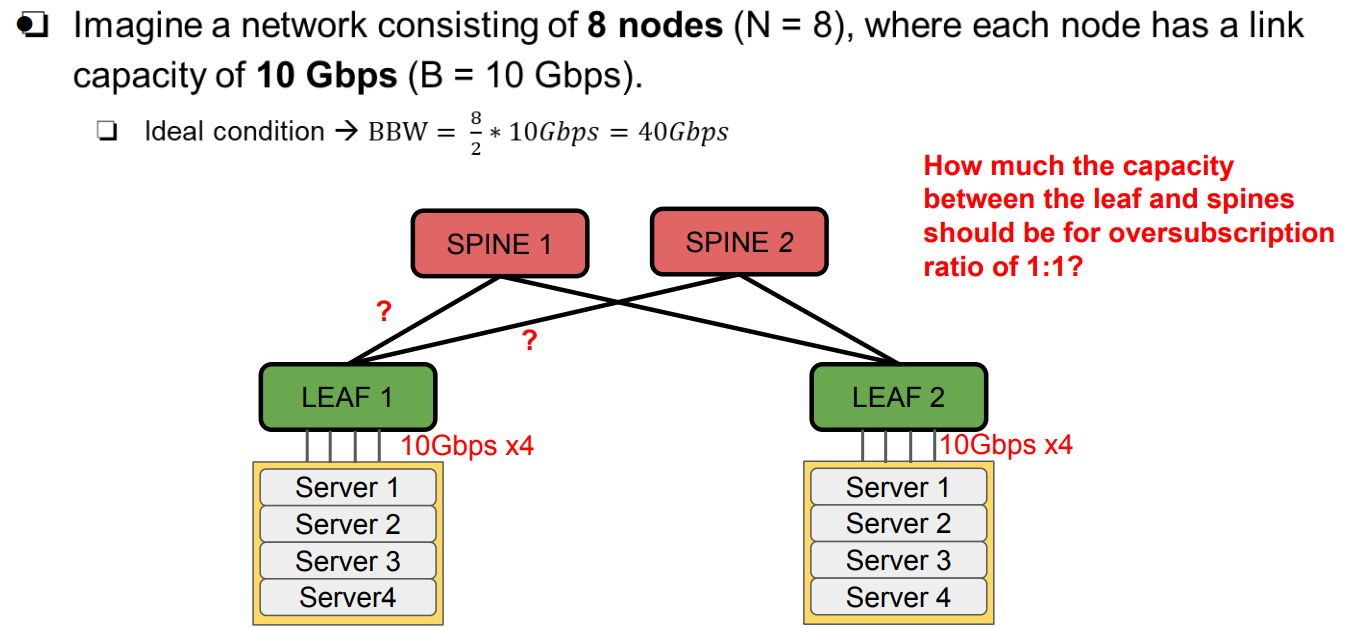
\includegraphics[width=0.68\textwidth]{immagini/NET_10/bandwidth_example.png}
\caption{Esempio di \emph{bisection bandwidth} e \emph{oversubscription}: per ottenere 1:1 l’uplink leaf$\rightarrow$spine deve eguagliare la capacità aggregata verso i server.}
\label{fig:net10-bisection-example}
\end{figure}

\paragraph{Connection to the external world}

La fabric leaf-spine è pensata per il traffico interno; l’accesso a Internet o a reti esterne viene spesso demandato a \emph{special leaves} (talvolta dette border/exit leaves) che concentrano le policy e gli uplink WAN/Internet. In pratica se ne impiegano almeno due per fault tolerance, evitando che la connettività esterna dipenda da un singolo dispositivo.


Riferimenti (slide + appunti) usati per il contenuto sopra: definizione dei tier ToR/EoR/Core e ruolo del core anche verso Internet ; limitazioni del basic tree (oversubscription, fault tolerance, costo dei tier alti) ; obiettivi delle reti DC e adozione di Clos/leaf-spine ; scalabilità e fault tolerance in leaf-spine (spine/leaf) ; LAG/MLAG, latenza (diametro), bisection bandwidth/oversubscription ed exit leaves

\subsubsection{Three-tier Clos: Fat Tree topology}

\paragraph{Fat Tree topology}
La \emph{fat-tree} è una topologia \emph{Clos} a \textbf{tre tier} che estende la leaf-spine aggiungendo un ulteriore livello gerarchico. In altre parole, rispetto al caso a due tier, la fat-tree introduce una separazione più esplicita tra \emph{edge/access} (dove si attestano i server), \emph{aggregation} e \emph{core/spine}, ottenendo una fabric più modulare e scalabile.

Un modo intuitivo per interpretarla (come nelle slide) è vedere una leaf “\emph{esplosa}” in un piccolo gruppo di leaf: questo gruppo prende il nome di \emph{pod}. In pratica, un \emph{pod} contiene tipicamente più switch di edge (verso i rack) e più switch di aggregation (verso il core), e replica questo schema in modo ripetibile per far crescere il data center per “blocchi”.

\paragraph{Example of Fat Tree topology}
Nell’esempio mostrato, ogni pod è composto da \textbf{quattro leaf} (indicate come 1a, 1b, 1c, 1d per il Pod 1; analogamente per gli altri), e sopra ai pod è presente un insieme di \textbf{spine/core} che interconnette tutti i pod. I server (o i rack) si attestano sugli switch di edge all’interno dei singoli pod; il traffico che deve uscire dal pod risale verso l’aggregation e poi viene instradato verso il core, che fornisce connettività uniforme verso gli altri pod.

Questo schema rende evidente il principio Clos: molti dispositivi relativamente “semplici” e ripetibili, con interconnessioni ridondate tra livelli, così da avere più cammini disponibili tra sorgente e destinazione. :contentReference[oaicite:3]{index=3}
\begin{figure}[H]
\centering
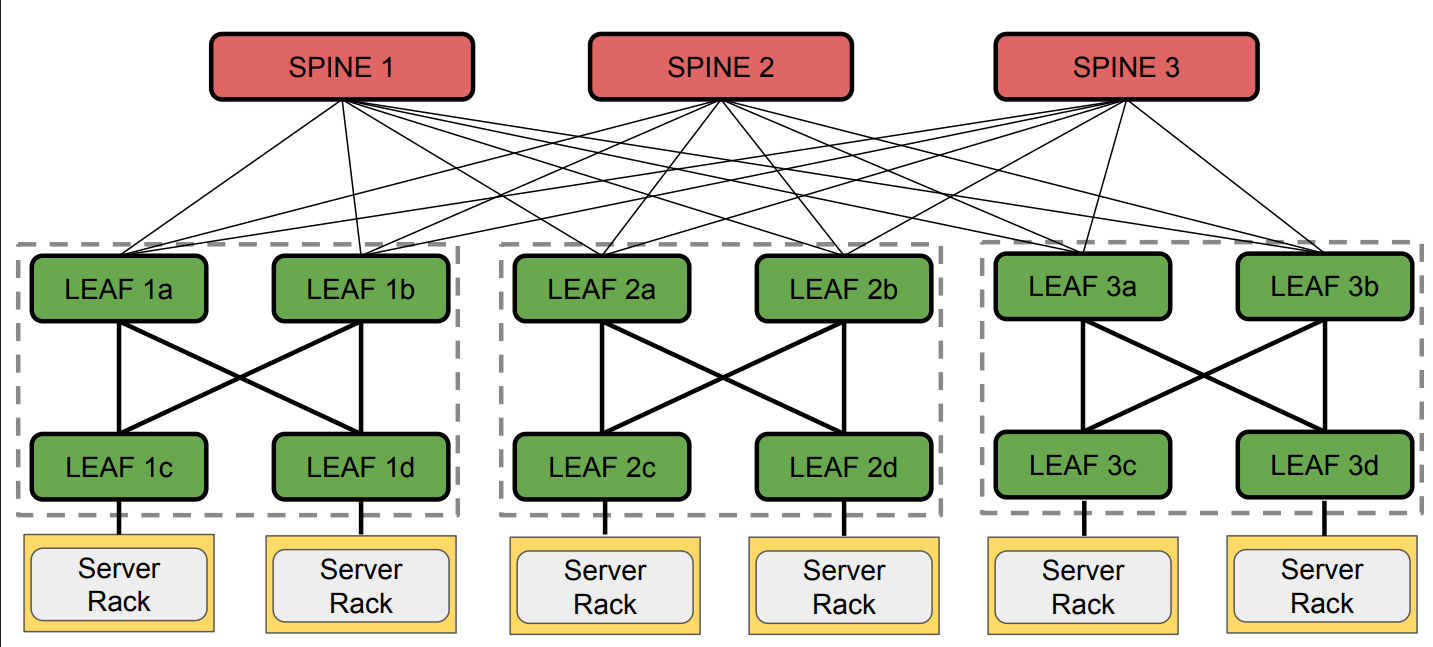
\includegraphics[width=0.86\textwidth]{immagini/NET_10/fat_tree_example.png}
\caption{Esempio di \emph{fat-tree} (Clos a tre tier): i \emph{pod} contengono edge+aggregation e sono interconnessi dal core/spine, creando molti cammini ridondanti tra rack.}
\label{fig:net10-fat-tree-example}
\end{figure}

\paragraph{Fat Tree: properties}
Le proprietà più rilevanti della fat-tree (e il motivo per cui è usata come architettura di riferimento nei DC di grandi dimensioni) sono:
\begin{itemize}
  \item \textbf{Scalabilità elevata}: con switch da 48 porte si può arrivare a \textbf{oltre 27k end-nodes} mantenendo una struttura regolare. :contentReference[oaicite:4]{index=4}
  \item \textbf{Full bisection bandwidth}: la topologia è progettata per mantenere \emph{bisection bandwidth} elevata (idealmente “piena”), quindi con buona capacità anche in scenari di traffico est-ovest intenso.
  \item \textbf{Uso di commodity switches}: invece di pochi apparati estremamente costosi, si impiegano switch più economici e numerosi, ottenendo ridondanza e capacità tramite la struttura della fabric.
  \item \textbf{Compatibilità con lo stack Ethernet/IP/TCP}: l’architettura resta compatibile con le soluzioni standard basate su Ethernet e IP, semplificando l’integrazione con l’ecosistema esistente. :contentReference[oaicite:7]{index=7}
\end{itemize}
\subsubsection{From L2 forwarding to network virtualization}

\paragraph{Packet Forwarding: from L2 to VXLAN}
Nelle fabric Clos di data center, l’approccio moderno consiste nel separare chiaramente \emph{underlay} e \emph{overlay}: l’underlay è una rete \textbf{L3 instradata} che garantisce connettività e multipath, mentre l’overlay realizza \textbf{semantiche L2/L3 virtuali} per i tenant sopra l’underlay. In questo contesto, \emph{VXLAN} (RFC~7348) è il meccanismo di riferimento: incapsula frame Ethernet (L2) in datagrammi \textbf{IP/UDP}, così che il trasporto avvenga come normale traffico IP e possa beneficiare dei meccanismi di routing e load balancing della rete sottostante.

L’incapsulamento/decapsulamento è demandato ai soli nodi di \emph{edge}, detti \emph{VTEP} (VXLAN Tunnel End Point): tipicamente i leaf (oppure, in alcuni scenari, direttamente gli end-host). La rete intermedia (spine e resto dell’underlay) vede pacchetti IP/UDP e non deve comprendere i dettagli dell’overlay.
Il campo chiave è il \emph{VNI} (VXLAN Network Identifier) a \textbf{24 bit}, che consente oltre \textbf{16 milioni} di domini virtuali, superando i limiti di scalabilità delle VLAN tradizionali; nel formato del pacchetto VXLAN, il VNI è trasportato nell’header VXLAN dopo l’UDP esterno (porta di destinazione tipicamente 4789).

\paragraph{L2 forwarding in Clos: why it does not scale}
Realizzare un grande dominio di forwarding L2 “puro” sopra una Clos non scala per motivi sia tecnici sia operativi. In primo luogo, per evitare loop a livello 2 è necessario lo \emph{Spanning Tree Protocol}, che tende a selezionare un solo cammino attivo per destinazione (in termini di forwarding verso MAC), rendendo di fatto \textbf{inefficace il load balancing} su una fabric con molti percorsi equivalenti.
In secondo luogo, la virtualizzazione basata su VLAN non è sufficiente in un contesto cloud: gli identificatori VLAN disponibili sono \textbf{meno di 4k}, troppo pochi per ambienti multi-tenant su larga scala.

A questi limiti si aggiunge l’impatto del traffico di controllo e del flooding tipico dei domini L2 (es. ARP e MAC learning in assenza di informazioni note), che in architetture estese può portare a repliche su ampia scala e a overhead non trascurabile nell’overlay; è uno dei motivi per cui, in seguito, viene introdotto un control plane (EVPN) per ridurre flooding e apprendimento basato su broadcast.

\paragraph{Network virtualization requirements}
La \emph{network virtualization} in ambito cloud nasce per soddisfare requisiti che la rete fisica, da sola, non può garantire con sufficiente flessibilità:
(i) \textbf{isolamento del traffico} (un tenant deve vedere solo i pacchetti della propria rete virtuale);
(ii) \textbf{riuso degli indirizzi} non solo a livello IP (subnet private riutilizzabili), ma anche a livello \textbf{MAC} (VM diverse, in reti virtuali diverse, possono avere MAC uguali);
(iii) \textbf{elasticità e mobilità} delle VM, che richiede di mantenere connettività e policy anche quando workload si spostano tra host/rack.

Questi vincoli implicano che i frame L2 dei tenant non debbano “vivere” direttamente nella fabric fisica, ma debbano essere \textbf{tunnelizzati} attraverso l’underlay (tipicamente L3): in questo modo la rete fisica resta semplice (routing IP e multipath), mentre l’overlay fornisce ai tenant l’illusione di switch/segmenti dedicati, con un numero di domini virtuali compatibile con la scala dei data center moderni.

\subsection{VXLAN}


\subsubsection{VXLAN comes to the rescue}

VXLAN (\emph{Virtual eXtensible Local Area Network}, RFC 7348) viene introdotto per rendere praticabile la virtualizzazione di rete in data center su larga scala: invece di estendere domini Layer 2 “fisici” (con i limiti di spanning tree e di scalabilità delle VLAN), VXLAN incapsula frame Ethernet (L2) in datagrammi IP/UDP, permettendo di trasportare connettività L2 sopra un underlay L3 instradato.


Il vantaggio principale è duplice. Da un lato, il VXLAN Network Identifier (VNI) è lungo 24 bit, quindi consente più di 16 milioni di domini logici (broadcast domain) e supera il vincolo delle VLAN tradizionali. Dall’altro, poiché l’overlay viaggia come traffico IP/UDP, l’underlay può usare routing e multipath (es. ECMP) per bilanciare i flussi. Inoltre, solo i nodi “edge” devono supportare l’incapsulamento: il resto della fabric vede semplici pacchetti IP.


\subsubsection{VXLAN in action}

Gli estremi dei tunnel VXLAN sono i \emph{VTEP} (\emph{VXLAN Tunnel End Point}): dispositivi che eseguono encap/decap e instaurano/terminano i tunnel VXLAN. Nelle architetture leaf-spine, tipicamente i VTEP coincidono con gli switch leaf (edge) che connettono i server/VM; l’underlay tra leaf e spine resta puramente L3 e instrada i pacchetti VXLAN come normale traffico IP.


Operativamente, quando un host invia un frame verso una destinazione appartenente allo stesso dominio virtuale, il leaf di ingresso (ingress VTEP) mappa il dominio L2 (es. VLAN/bridge) su un VNI, incapsula il frame originale e invia il pacchetto nell’underlay verso l’egress VTEP (identificato dal suo indirizzo IP). L’egress VTEP rimuove gli header esterni e inoltra il frame originale verso il server di destinazione.


Un dettaglio importante è che i VTEP possono essere implementati anche sugli end-host (ad esempio nel virtual switch dell’hypervisor), ma il processamento software dell’encapsulamento può essere oneroso se non supportato in hardware dalla NIC; viceversa, gli switch leaf moderni includono spesso supporto hardware per VXLAN a line-rate.

\begin{figure}[H]
\centering
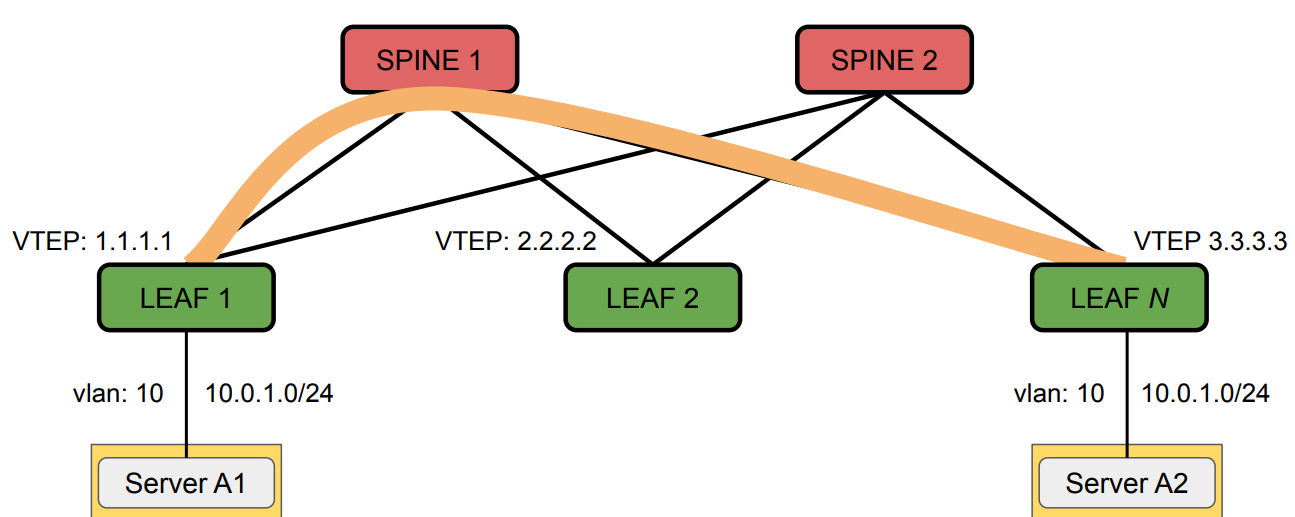
\includegraphics[width=0.82\textwidth]{immagini/NET_10/vxlan_in_action.png}
\caption{VXLAN in azione: i leaf agiscono da VTEP e incapsulano frame L2 del tenant in pacchetti IP/UDP instradati nell’underlay L3 tra leaf e spine.}
\label{fig:net10-vxlan-action}
\end{figure}

\subsubsection{VXLAN packet format}

Il pacchetto VXLAN è composto da un frame Ethernet “interno” (originale) incapsulato in un insieme di header esterni: \emph{Outer L2 header} (per il forwarding sul link locale dell’underlay), \emph{Outer IP header} (con sorgente = IP del VTEP di ingresso e destinazione = IP del VTEP di uscita), \emph{Outer UDP header} e infine \emph{VXLAN header}, che trasporta il VNI.


Nel formato mostrato a lezione, la porta UDP di destinazione è fissata (4789), mentre la porta sorgente è variabile. Questo non è un dettaglio “cosmetico”: in una fabric Clos, l’ECMP viene calcolato sulla 5-tuple degli header esterni (src/dst IP, src/dst port, protocollo). Poiché molti campi del tunnel (in particolare src/dst IP e dst port) restano costanti tra una coppia di VTEP, la variabilità della UDP source port consente di distribuire i flussi su più percorsi; in pratica l’ingress VTEP sceglie la porta sorgente come funzione hash del pacchetto interno.

\begin{figure}[H]
\centering
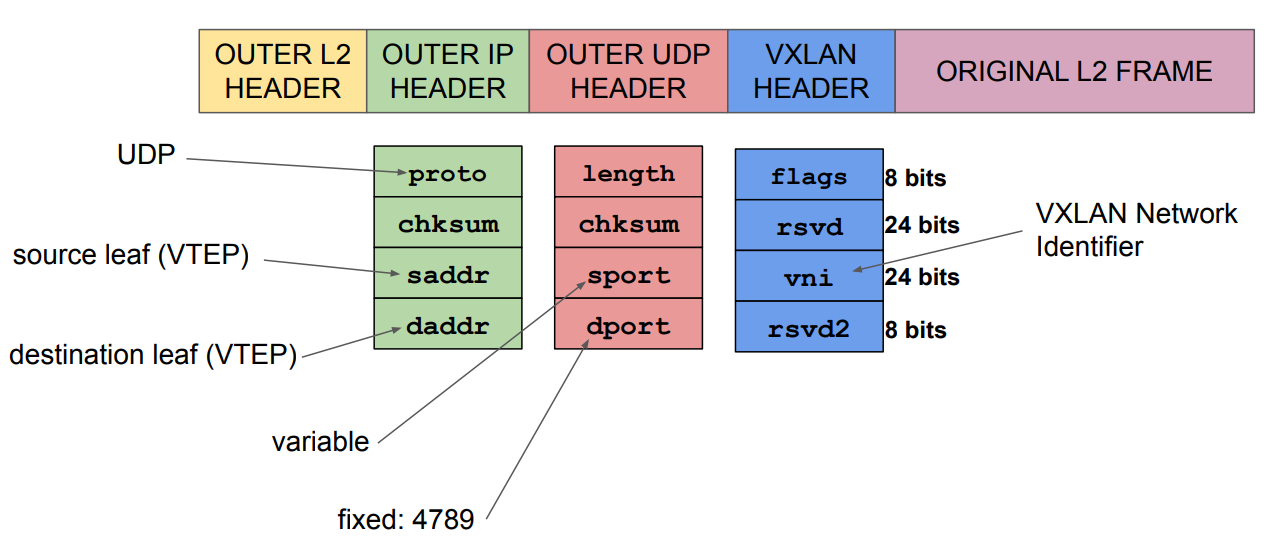
\includegraphics[width=0.7\textwidth]{immagini/NET_10/vxlan_packet_format.png}
\caption{Formato del pacchetto VXLAN: il frame Ethernet originale è incapsulato con header esterni Ethernet/IP/UDP e header VXLAN che trasporta il VNI (24 bit).}
\label{fig:net10-vxlan-format}
\end{figure}

\subsubsection{L2VNI vs L3VNI}

Si distinguono due utilizzi principali del VNI.

Un \textbf{L2VNI} identifica un dominio di broadcast Layer 2: è il VNI associato a un singolo \emph{Broadcast Domain} (BD) di uno specifico tenant (tipicamente equivalente “logico” di una VLAN/bridge nel contesto di quel tenant).


Un tenant, però, può avere più subnet e richiedere comunicazione \emph{inter-subnet}. In questo caso si introduce un \textbf{L3VNI}, usato per il routing Layer 3 tra più L2VNI dello stesso tenant: l’L3VNI è (di norma) associato uno-a-uno a una VRF del tenant, e all’interno della stessa VRF possono coesistere molteplici L2VNI.


\subsubsection{L2VNI vs L3VNI (example)}

Nell’esempio delle slide, lo stesso tenant possiede due domini L2 distinti (ad esempio VLAN 10 e VLAN 20) con subnet differenti (10.0.1.0/24 e 10.0.0.0/24). I due domini di broadcast sono mappati su due L2VNI diversi (ad esempio L2VNI 101 e L2VNI 102): il traffico “intra-subnet” resta confinato nel rispettivo L2VNI e viene trasportato come overlay L2 sopra l’underlay L3.


Per permettere che host della subnet 10.0.1.0/24 comunichino con host della subnet 10.0.0.0/24, il tenant introduce una VRF comune e un L3VNI (nell’esempio, L3VNI 100) presente sui leaf coinvolti. In questo modo, quando un pacchetto deve attraversare domini di broadcast diversi dello stesso tenant, il forwarding avviene a livello 3 all’interno della VRF (overlay L3), mantenendo comunque isolati tenant e tabelle di routing rispetto ad altri clienti.
\begin{figure}[H]
\centering
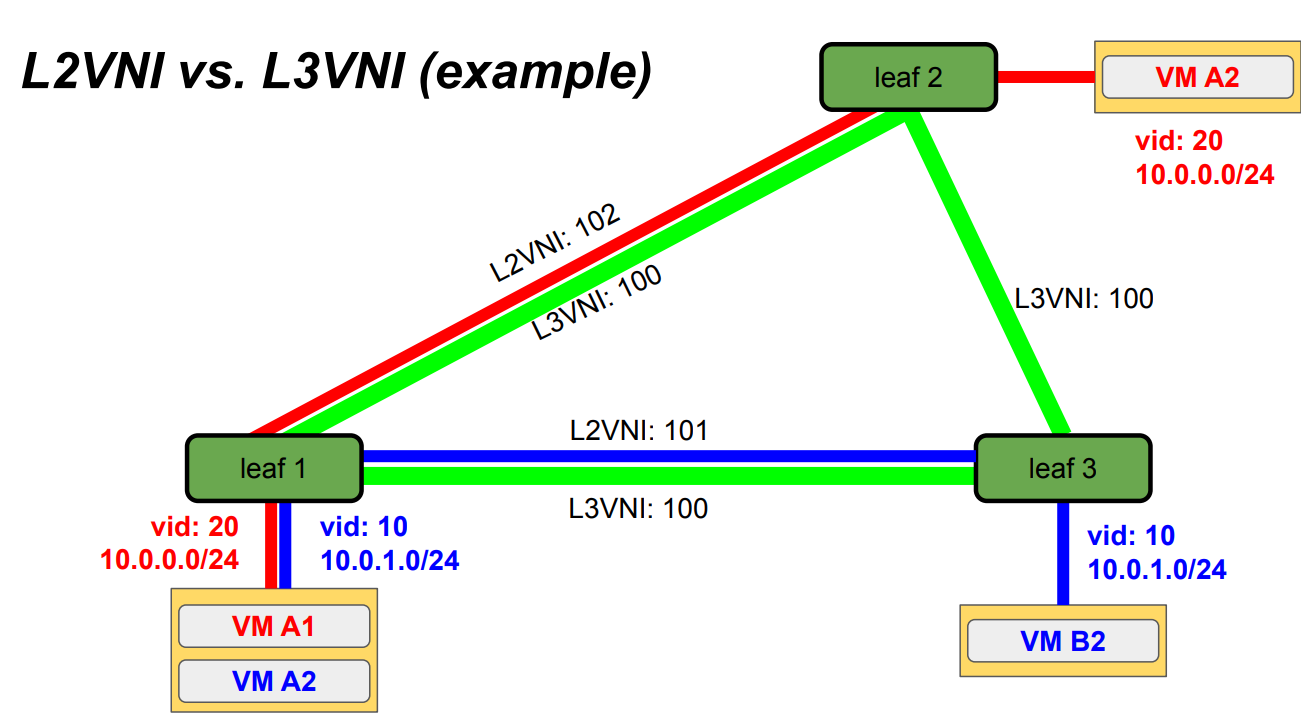
\includegraphics[width=0.88\textwidth]{immagini/NET_10/l2vni_l3vni_example.png}
\caption{Esempio L2VNI/L3VNI: due domini L2 (due subnet, due L2VNI) appartenenti allo stesso tenant condividono una VRF comune; l’L3VNI abilita routing tra subnet nella stessa VRF.}
\label{fig:net10-l2vni-l3vni-example}
\end{figure}

\subsubsection{Forwarding behavior (example in leaf-spine)}

Per fissare le idee, consideriamo il caso mostrato nelle slide: una VM invia traffico verso un’altra VM dello stesso tenant, quindi l’host trasmette a livello 2 (frame Ethernet) su una VLAN di accesso. Il punto chiave è che, nella fabric, il traffico viene trasportato come VXLAN sopra un underlay L3, quindi il forwarding effettivo attraversa leaf e spine come normale traffico IP/UDP. \textbf{Non} si configura un tunnel per ogni possibile cammino: il tunnel è tra VTEP, mentre la scelta del percorso avviene dinamicamente nell’underlay (ECMP).

\paragraph{Ingress leaf (ingress VTEP)}
Quando il frame entra sul leaf di accesso, il leaf esegue tipicamente queste operazioni:
\begin{enumerate}
  \item individua l’interfaccia VXLAN (e quindi il \emph{VNI}) associata alla VLAN di accesso del tenant;
  \item incapsula il frame originale aggiungendo gli header esterni (outer Ethernet/IP/UDP + VXLAN), impostando IP sorgente/destinazione sugli indirizzi dei VTEP (leaf di ingresso e leaf di uscita) e scegliendo la \emph{UDP source port} in modo da introdurre entropia (tipicamente come funzione dell’inner flow);
  \item inoltra il pacchetto nell’underlay verso il \emph{next-hop} selezionato dai meccanismi di multipath (ECMP) sulla base degli header esterni.
\end{enumerate}

\paragraph{Underlay (spine)}
Il pacchetto VXLAN viene instradato nella fabric come un comune traffico IP/UDP: lo spine riceve il pacchetto e lo inoltra verso il leaf di destinazione scelto, mantenendo la semantica L3 dell’underlay.

\paragraph{Egress leaf (egress VTEP)}
Arrivato al leaf di destinazione, il dispositivo:
\begin{enumerate}
  \item riconosce che il pacchetto è VXLAN destinato al VTEP locale;
  \item rimuove gli header esterni (decapsulamento);
  \item inoltra il frame interno sulla porta/bridge del tenant verso il server di destinazione.
\end{enumerate}


\subsubsection{ECMP and load balancing}

\paragraph{Load balancing: ECMP}
Le topologie Clos (leaf-spine / fat-tree) offrono, per costruzione, \emph{molteplici cammini equivalenti} tra sorgente e destinazione. Per sfruttarli davvero, il bilanciamento deve avvenire a \textbf{Layer 3}, dove la rete può distribuire i flussi su link diversi mantenendo al contempo proprietà di stabilità e prevedibilità. Una delle soluzioni più usate è \emph{ECMP} (\emph{Equal Cost MultiPath routing}): l’idea è calcolare un \textbf{hash della 5-tuple} del pacchetto (indirizzi IP sorgente/destinazione, porte sorgente/destinazione, protocollo) e usare il risultato per selezionare uno dei next-hop a costo uguale. Il valore dell’hash viene tipicamente mappato in \emph{hash buckets} associati ai diversi next-hop disponibili, così da ottenere una distribuzione “abbastanza uniforme” dei flussi. :contentReference[oaicite:0]{index=0}

L’uso dell’hash (invece di soluzioni più semplici come round robin) è motivato da un vincolo prestazionale fondamentale nei data center: \textbf{i pacchetti dello stesso flusso devono seguire lo stesso cammino}, altrimenti si rischia ricezione fuori ordine (ad esempio su TCP), con impatto negativo sulle performance complessive. :contentReference[oaicite:1]{index=1}
\begin{figure}[H]
\centering
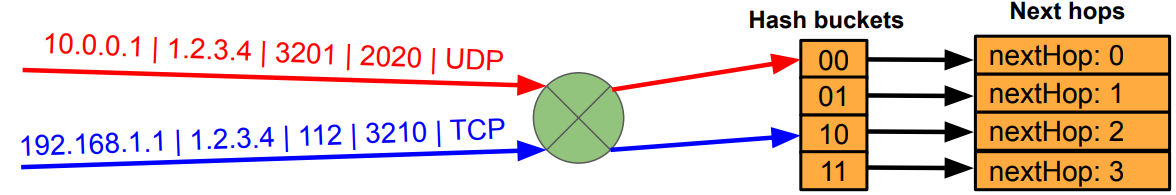
\includegraphics[width=0.88\textwidth]{immagini/NET_10/ecmp_hash_buckets.png}
\caption{ECMP: selezione del next-hop tramite hash della 5-tuple, mappato su \emph{hash buckets}. I pacchetti dello stesso flusso restano sullo stesso percorso per evitare reordering.}
\label{fig:net10-ecmp-buckets}
\end{figure}

\paragraph{VXLAN and ECMP}
Nel caso VXLAN, l’underlay è una rete L3 che deve poter fare ECMP \emph{anche senza “capire” VXLAN}: non tutti i nodi dell’underlay (es. spine) eseguono encap/decap, quindi il calcolo ECMP avviene \textbf{sulla 5-tuple degli header esterni} (outer IP/UDP). :contentReference[oaicite:2]{index=2}
Il problema è che la 5-tuple del tunnel VXLAN, a parità di coppia ingress/egress VTEP, sarebbe quasi sempre costante: IP sorgente = VTEP di ingresso, IP destinazione = VTEP di uscita, protocollo = UDP, UDP destination port = porta VXLAN. L’unico campo che può variare “a comando” è la \textbf{UDP source port}. Per questo l’ingress VTEP sceglie la UDP source port come funzione hash del pacchetto interno (inner 5-tuple), inserendo entropia nel traffico esterno e rendendo efficace la distribuzione ECMP sui percorsi disponibili.
Di conseguenza, non è necessario configurare “un tunnel per ogni percorso”: si configura il tunnel tra VTEP (terminazioni), mentre l’underlay seleziona dinamicamente il cammino tramite ECMP.

\subsubsection{VXLAN VTEPs (NIC and switches)}
I \emph{VTEP} (\emph{VXLAN Tunnel End Points}) sono le terminazioni dei tunnel VXLAN: i nodi che effettuano \textbf{incapsulamento e decapsulamento} e che, in una fabric leaf-spine, coincidono spesso con gli switch \emph{leaf} (edge). Tuttavia, un VTEP può anche risiedere sugli \textbf{end-host}, cioè direttamente sui server. :contentReference[oaicite:5]{index=5}

Dal punto di vista prestazionale/implementativo, la collocazione è rilevante:
\begin{itemize}
  \item \textbf{VTEP su switch (leaf)}: gli switch moderni integrano supporto hardware per VXLAN, quindi l’operazione di encap/decap può avvenire a \emph{line-rate} con overhead ridotto. :contentReference[oaicite:6]{index=6}
  \item \textbf{VTEP su server/NIC}: non tutte le NIC supportano accelerazione hardware VXLAN; in assenza di offload, eseguire encap/decap in software può essere pesante. In pratica, l’hypervisor ospita spesso un \emph{virtual switch} che gestisce la virtualizzazione di rete e può terminare i tunnel a livello host. :contentReference[oaicite:7]{index=7}
\end{itemize}

\subsubsection{Why VXLAN and not e.g.\ MPLS?}
Un confronto “di principio” con MPLS chiarisce perché VXLAN è tipicamente preferito nei data center cloud. MPLS nasce con l’obiettivo di \textbf{velocizzare il forwarding} nel core tramite \emph{label switching}, non come meccanismo generale di \textbf{network virtualization}. Esistono tecnologie come \emph{VPLS} che estendono reti L2 usando il dataplane MPLS, ma non rappresentano un overlay IP “generico” nello stesso senso: MPLS rimane una rete \emph{switched} basata su label e, nella pratica, non è la scelta più comune per i data center moderni.

VXLAN, invece, è progettato esplicitamente per \textbf{incapsulare frame L2 su un underlay L3} (IP/UDP), quindi abilita la virtualizzazione a livello 2 “sopra qualunque rete IP”, mantenendo la fabric semplice e sfruttando nativamente routing e multipath. Per le esigenze cloud (multi-tenancy, isolamento, e soprattutto \textbf{mobilità delle VM}), VXLAN risulta quindi più aderente ai requisiti operativi del data center.
\subsection{EVPN}

\subsubsection{VXLAN control plane: Ethernet VPN (EVPN)}
VXLAN, così come descritto in RFC~7348, definisce il \emph{data plane} di incapsulamento ma \textbf{non} specifica un \emph{control plane}. In assenza di control plane, i tunnel VXLAN sono spesso configurati \emph{staticamente}: questo approccio non scala (espansione complessa) e, soprattutto, amplifica il traffico di \emph{flooding} nell’overlay (es. richieste ARP e MAC flooding replicate attraverso l’underlay).

\emph{Ethernet VPN (EVPN)} è introdotto proprio per colmare questa lacuna: è il \textbf{control plane per VXLAN} e consente di spostare nel piano di controllo parte dell’“apprendimento” tipico del Layer~2 (MAC learning e ARP), riducendo il flooding e automatizzando la costruzione dell’overlay.

\subsubsection{A control plane for VXLAN}
EVPN utilizza \textbf{MP-BGP} (lo stesso meccanismo già noto nelle VPN MPLS-BGP) introducendo una \textbf{nuova address family} per scambiare informazioni EVPN tra VTEP.
L’idea operativa è che ogni VTEP (terminazione del tunnel) esporti tramite BGP le informazioni relative ai tenant e alle reti/segmenti che ospita; gli altri VTEP importano tali annunci e possono quindi:
\begin{itemize}
  \item \textbf{scoprire automaticamente} gli altri VTEP rilevanti (discovery);
  \item \textbf{stabilire automaticamente} i tunnel VXLAN necessari;
  \item \textbf{ridurre il flooding} perché MAC learning e associazioni IP--MAC (ARP) vengono propagate in control plane anziché tramite broadcast nell’overlay;
  \item veicolare sia \textbf{informazioni L2} (MAC/IP) sia \textbf{informazioni L3} (routing/prefissi) in modo coerente con VRF e VNIs.
\end{itemize}


\subsubsection{EVPN message types}
EVPN definisce cinque tipologie di messaggi (route types) per scambiare informazioni:
\begin{itemize}
  \item \textbf{Type 1}: Ethernet Auto-Discovery (A-D) route
  \item \textbf{Type 2}: MAC/IP Advertisement route
  \item \textbf{Type 3}: Inclusive Multicast Ethernet Tag route
  \item \textbf{Type 4}: Ethernet Segment route
  \item \textbf{Type 5}: IP Prefix route
\end{itemize}
In questo contesto ci si concentra principalmente sui \textbf{type 2, 3 e 5}; i type 1 e 4 sono tipicamente legati a scenari avanzati di \emph{multi-homing} (es. identificazione di segmenti Ethernet via ESI per aumentare l’affidabilità lato accesso).

\subsubsection{EVPN Type 2}
Le route \textbf{EVPN Type 2} sono scambiate tra VTEP per \textbf{advertising di MAC e IP} degli host all’interno di uno specifico broadcast domain (quindi, tipicamente, di uno specifico \emph{L2VNI}). L’obiettivo è \textbf{sincronizzare} tra tutti i VTEP la \emph{FIB} (MAC table) e le associazioni IP--MAC (ARP table), sostituendo MAC learning e ARP request basati su flooding.

\paragraph{EVPN Type 2 format}
Il formato (campi principali) di una route Type~2 include (TULUX DICE CHE NON IMPORTA RICORDARSI TUTTI I SINGOLI CAMPI):
\begin{itemize}
  \item \textbf{Route Distinguisher (RD)}: identificatore dell’istanza EVPN (non necessariamente “uguale” all’uso che aveva nelle VPN MPLS-BGP).
  \item \textbf{Ethernet Segment ID (ESI)}: identificatore (avanzato) per scenari di multihoming/LAG.
  \item \textbf{Ethernet Tag ID}: tipicamente l’ID VLAN configurato sul dispositivo (associato al BD/L2VNI).
  \item \textbf{IP address length, IP address, GW address}: informazioni IP dell’host (o del gateway).
  \item \textbf{MPLS Label 1 / MPLS Label 2}: nei casi VXLAN trasportano gli identificatori VXLAN (VNIs), rispettivamente per L2VNI e L3VNI (3 byte $\rightarrow$ 24 bit).
  \item \textbf{MAC address length, MAC address}: MAC dell’host.
\end{itemize}


\paragraph{Type 2: Host MAC advertisement}
Nel caso più semplice (solo L2), le Type~2 servono a “insegnare” ai VTEP remoti i \textbf{MAC degli host} presenti dietro un VTEP: dopo il peering EVPN, ogni VTEP annuncia le proprie entry di forwarding (MAC learned) agli altri, realizzando di fatto il MAC learning via BGP anziché tramite flooding nell’overlay.

\paragraph{Type 2: Host ARP advertisement}
Una Type~2 può anche trasportare una entry \textbf{ARP} (associazione IP--MAC), abilitando \emph{host ARP advertisement} e quindi \textbf{ARP broadcast suppression}: quando un VTEP riceve informazioni ARP dagli host (ad esempio tramite gratuitous ARP), le annuncia agli altri VTEP; se in seguito riceve una richiesta ARP broadcast, può rispondere/convertire la richiesta in un unicast verso il MAC corretto invece di floodare nell’overlay.
Un secondo caso d’uso importante è la \textbf{VM migration}: spostando una VM dietro un altro VTEP, le nuove informazioni IP--MAC vengono annunciate; il VTEP precedente può rilevare la migrazione e, se necessario, ritirare le route obsolete.

\paragraph{Type 2: IP route advertisement}
Per la comunicazione Layer~3 tra host in subnet diverse, i VTEP devono scambiarsi anche \textbf{informazioni di reachability IP}. Nello scenario presentato, le Type~2 vengono usate per annunciare host route (tipicamente /32 o /128) e permettere ai VTEP di apprendere le reachability “dietro” ciascun VTEP in relazione alle L2VPN/L2VNI configurate. :contentReference[oaicite:10]{index=10}

\subsubsection{EVPN Type 3}

Le route \textbf{EVPN Type 3} (\emph{Inclusive Multicast Ethernet Tag}) servono principalmente a far sì che i VTEP si \textbf{scoprano} a vicenda per un determinato segmento L2 (quindi per un determinato \emph{L2VNI}) e possano costruire la \textbf{replication list} per il traffico \emph{BUM} (Broadcast, Unknown-unicast, Multicast).

In particolare, una Type~3 viene usata per:
\begin{itemize}
  \item \textbf{advertising di L2VNI e dell’IP del VTEP} (terminazione VXLAN) verso gli altri VTEP;
  \item \textbf{creazione della replication list}: i VTEP che ricevono l’annuncio sanno che quel peer partecipa a quel broadcast domain e quindi può dover ricevere traffico BUM di quel segmento;
  \item \textbf{discovery e tunnel establishment dinamico}: quando un VTEP riceve una Type~3 relativa a un L2VNI configurato localmente, può impostare automaticamente un tunnel VXLAN verso il VTEP remoto (senza configurazioni statiche punto-punto).
\end{itemize}

Nelle slide questa logica è collegata al fatto che l’informazione di multicast/replicazione viene veicolata tramite una BGP Extended Community chiamata \textbf{PMSI} (\emph{P-Multicast Service Interface}), che porta i dettagli utili per la distribuzione del traffico BUM nell’overlay.

\paragraph{EVPN Type 3 format}
Nel formato mostrato a lezione, i campi rilevanti di una Type~3 includono:
\begin{itemize}
  \item \textbf{Route Distinguisher (RD)};
  \item \textbf{Ethernet Tag ID} (identifica il segmento/VLAN locale associato al BD);
  \item \textbf{IP address length} e \textbf{Originating IP address}, cioè l’indirizzo IP del \emph{VTEP} che origina la route (informazione chiave per la discovery);
  \item \textbf{Flags}: informazioni addizionali, tipicamente non utilizzate nel caso VXLAN;
  \item \textbf{Tunnel Type}: identifica la tecnologia di tunnel (nelle slide, per VXLAN è indicato con valore 6);
  \item \textbf{MPLS label}: nel contesto VXLAN è usato per trasportare l’identificatore del servizio, cioè l’\textbf{L2VNI};
  \item \textbf{Tunnel Identifier}: contiene informazioni sul tunnel e include anche l’indirizzo del VTEP.
\end{itemize}
\subsubsection{EVPN Type 5}

Le route \textbf{EVPN Type 5} (\emph{IP Prefix route}) sono usate per distribuire \textbf{prefissi IP} (non solo host route /32 o /128) tra i VTEP e fornire informazione di \textbf{reachability a livello L3} \emph{associata a una L3VNI} (quindi alla \emph{VRF} del tenant), non ai singoli broadcast domain (L2VNI).

Nelle slide è evidenziato il parallelismo con le Type~2: una Type~2 può annunciare host route (tipicamente /32), mentre una Type~5 permette di annunciare \textbf{subnet con lunghezza di prefisso variabile}. Di conseguenza, le Type~5 sono lo strumento principale per abilitare \textbf{inter-subnet routing} tra più L2VNI appartenenti allo stesso tenant, mantenendo l’isolamento della tabella di routing dentro la VRF del tenant.

\begin{figure}[H]
\centering
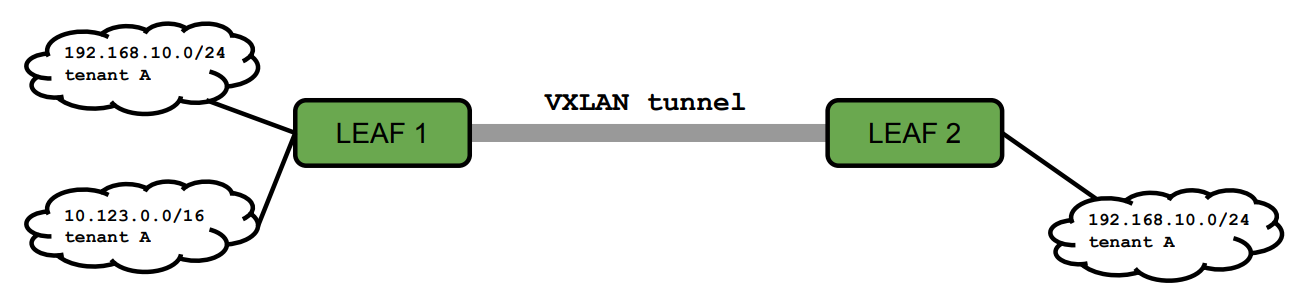
\includegraphics[width=0.82\textwidth]{immagini/NET_10/evpn_type5_concept.png}
\caption{EVPN Type 5 (IP Prefix route): distribuzione di prefissi con lunghezza variabile a livello VRF/L3VNI, abilitando routing inter-subnet tra più L2VNI dello stesso tenant.}
\label{fig:net10-evpn-type5-concept}
\end{figure}


\paragraph{EVPN Type 5 format}
Il formato mostrato nelle slide include campi analoghi a quelli già visti, con in evidenza le informazioni L3:
\begin{itemize}
  \item \textbf{Route Distinguisher (RD)};
  \item \textbf{Ethernet Segment ID (ESI)} e \textbf{Ethernet Tag ID} (presenti anche se, nel caso d’uso VXLAN più comune, l’interesse principale è la reachability IP in VRF);
  \item \textbf{IP address length} e \textbf{IP address}: prefisso IP annunciato (non necessariamente /32);
  \item \textbf{GW address}: indirizzo gateway associato all’annuncio;
  \item \textbf{MPLS label(s)}: nel contesto VXLAN veicolano gli identificatori di servizio coerenti con VNIs (L2/L3) dell’istanza;
  \item opzionalmente \textbf{MAC address length} e \textbf{MAC address}.
\end{itemize}

{\LARGE \textbf{Laboratorio}} \\[0.5em]
\subsection{Laboratorio: VXLAN + EVPN con MP-BGP su fabric leaf-spine (L2VPN + estensione L3VNI)}

\paragraph{Obiettivo.}
Questo laboratorio mostra come realizzare una fabric \emph{leaf-spine} con:
\begin{itemize}
    \item \textbf{underlay L3} instradato (convergenza e connettività tra i VTEP);
    \item \textbf{overlay VXLAN} per due tenant distinti (L2VNI);
    \item \textbf{control plane EVPN} basato su \textbf{MP-BGP} per eliminare (o ridurre drasticamente) flooding e apprendimento L2 distribuito;
    \item \textbf{estensione opzionale} con \textbf{L3VNI} e pubblicazione di \textbf{prefissi (Type 5)}.
\end{itemize}

\paragraph{Strumenti.}
\begin{itemize}
    \item \textbf{GNS3} (o ambiente equivalente) per emulare la topologia leaf-spine.
    \item \textbf{FRRouting (FRR)} per OSPF (underlay) e MP-BGP EVPN (control plane).
    \item \textbf{Linux networking} su leaf: \texttt{iproute2}, \texttt{bridge}, interfacce \texttt{vxlan}, VRF Linux, bridge VLAN-aware.
\end{itemize}

\paragraph{Scenario (alto livello).}
\begin{itemize}
    \item Tre leaf (\textbf{L1}, \textbf{L2}, \textbf{L3}) che fungono da \textbf{VTEP}.
    \item Due spine (\textbf{S1}, \textbf{S2}) per l'underlay L3.
    \item \textbf{Tenant A}: VLAN 10, subnet \texttt{10.0.10.0/24}, trasportata su \textbf{L2VNI 110}.
    \item \textbf{Tenant B}: VLAN 20, subnet \texttt{10.0.20.0/24}, trasportata su \textbf{L2VNI 120}.
    \item VTEP loopback (esempio coerente con le slide):
    \begin{itemize}
        \item L1: \texttt{100.64.0.1/32} \qquad L2: \texttt{100.64.0.2/32} \qquad L3: \texttt{100.64.0.3/32}
        \item S1: \texttt{100.64.0.10/32} \qquad S2: \texttt{100.64.0.11/32}
    \end{itemize}
    \item MP-eBGP EVPN:
    \begin{itemize}
        \item Spine in \textbf{AS 65000}, leaf in \textbf{AS 65001/65002/65003}.
    \end{itemize}
\end{itemize}

\begin{figure}[H]
\centering
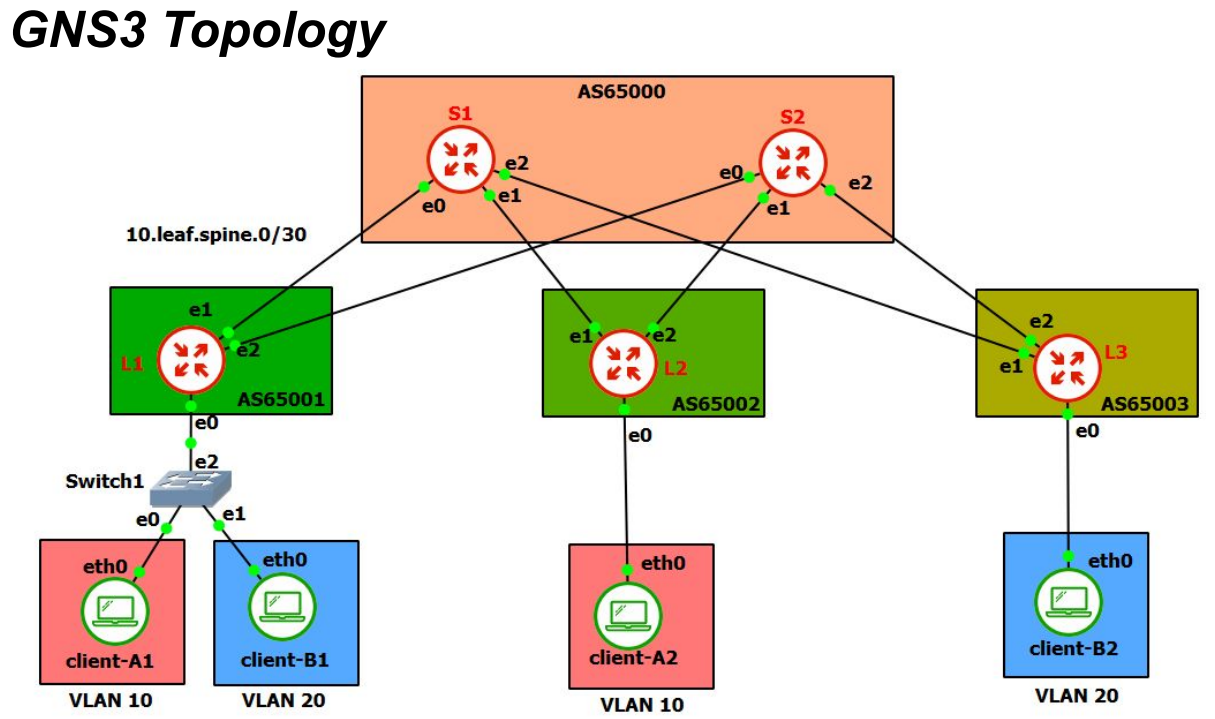
\includegraphics[width=0.86\textwidth]{immagini/NET_10/lab_gns3_topology.png}
\caption{Topologia di laboratorio in GNS3: fabric leaf-spine con due spine (AS65000) e tre leaf (VTEP) connessi a host dei tenant su VLAN 10 e VLAN 20.}
\label{fig:net10-lab-topology}
\end{figure}

\subsubsection{Avvio dell'emulazione e controlli preliminari}

\paragraph{Step 0: avvio topologia e accesso ai nodi.}
Avviare la topologia e aprire una shell su L1/L2/L3 e sui due spine S1/S2. Verificare la connettività di base sui link direttamente connessi (ping tra interfacce adiacenti).

\paragraph{Step 1: verifica che FRR sia operativo.}
Su ciascun router (leaf e spine) verificare accesso a \texttt{vtysh} e configurazione di base.
\begin{verbatim}
vtysh
show running-config
\end{verbatim}

\subsubsection{Fase 1: Underlay L3 (indirizzamento + OSPF)}

\paragraph{Step 2: configurare gli indirizzi IP dell'underlay (FRR).}
Configurare gli IP sulle interfacce leaf--spine (p2p /30) e sulle loopback (VTEP /32).
\emph{Nota:} la mappatura precisa interfaccia/IP dipende dalla tua topologia GNS3; l'obiettivo è replicare lo schema delle slide.

\begin{verbatim}
! Esempio (da adattare alle interfacce del tuo scenario):
interface eth1
 ip address 10.1.1.1/30
interface eth2
 ip address 10.1.2.1/30
interface lo
 ip address 100.64.0.1/32
\end{verbatim}

\paragraph{Step 3: configurare OSPF sull'underlay.}
Abilitare OSPF su link p2p e annunciare anche le loopback dei VTEP.
\begin{verbatim}
router ospf
 ospf router-id 100.64.0.1
 network 10.1.1.0/30 area 0
 network 10.1.2.0/30 area 0
 network 100.64.0.1/32 area 0
\end{verbatim}

\paragraph{Step 4: verifiche OSPF e reachability tra VTEP.}
Controllare che le adiacenze OSPF siano \emph{Full} e che ogni leaf raggiunga le loopback degli altri leaf.
\begin{verbatim}
show ip ospf neighbor
show ip route ospf
ping 100.64.0.2
ping 100.64.0.3
\end{verbatim}

\subsubsection{Fase 2: Overlay VXLAN (L2VNI) lato leaf: VRF + bridge + VNI}

\paragraph{Step 5: configurare L1 (tenant A + tenant B).}
Su L1 impostare l'IP VTEP su loopback, creare VRF e bridge per ciascun tenant, mappare la VLAN di accesso su una sub-interfaccia e creare il device VXLAN (\texttt{vni110} e \texttt{vni120}).

\begin{verbatim}
# vtep IP address
ip addr add 100.64.0.1/32 dev lo

# -------------------------
# tenant A (VLAN 10, L2VNI 110)
ip link add vrf1 type vrf table 1100
ip link set vrf1 up

ip link add br10 type bridge
ip link set br10 master vrf1
ip link set br10 addr aa:bb:cc:00:00:01
ip addr add 10.0.10.1/24 dev br10    # SVI (gateway tenant A)

ip link add link eth0 name eth0.10 type vlan id 10
ip link set eth0.10 master br10
ip link set eth0.10 up
ip link set br10 up

ip link add vni110 type vxlan local 100.64.0.1 dstport 4789 id 110 nolearning
ip link set vni110 master br10 addrgenmode none
ip link set vni110 type bridge_slave neigh_suppress on learning off
ip link set vni110 up

# -------------------------
# tenant B (VLAN 20, L2VNI 120)
ip link add vrf2 type vrf table 1200
ip link set vrf2 up

ip link add br20 type bridge
ip link set br20 master vrf2
ip link set br20 addr aa:bb:cc:00:00:11
ip addr add 10.0.20.1/24 dev br20    # SVI (gateway tenant B)

ip link add link eth0 name eth0.20 type vlan id 20
ip link set eth0.20 master br20
ip link set eth0.20 up
ip link set br20 up

ip link add vni120 type vxlan local 100.64.0.1 dstport 4789 id 120 nolearning
ip link set vni120 master br20 addrgenmode none
ip link set vni120 type bridge_slave neigh_suppress on learning off
ip link set vni120 up
\end{verbatim}

\paragraph{Step 6: configurare L2 (solo tenant A) e L3 (solo tenant B).}
Replicare lo schema su L2 per VLAN10/L2VNI110 e su L3 per VLAN20/L2VNI120 (con i rispettivi VTEP \texttt{100.64.0.2} e \texttt{100.64.0.3}).

\begin{verbatim}
# L2: tenant A (estratto)
ip addr add 100.64.0.2/32 dev lo
ip link add vrf1 type vrf table 1100
ip link set vrf1 up
ip link add br10 type bridge
ip link set br10 master vrf1
ip link set br10 addr aa:bb:cc:00:00:02
ip addr add 10.0.10.1/24 dev br10
ip link add link eth0 name eth0.10 type vlan id 10
ip link set eth0.10 master br10
ip link set eth0.10 up
ip link set br10 up
ip link add vni110 type vxlan local 100.64.0.2 dstport 4789 id 110 nolearning
ip link set vni110 master br10 addrgenmode none
ip link set vni110 type bridge_slave neigh_suppress on learning off
ip link set vni110 up

# L3: tenant B (estratto)
ip addr add 100.64.0.3/32 dev lo
ip link add vrf2 type vrf table 1200
ip link set vrf2 up
ip link add br20 type bridge
ip link set br20 master vrf2
ip link set br20 addr aa:bb:cc:00:00:33
ip addr add 10.0.20.1/24 dev br20
ip link add link eth0 name eth0.20 type vlan id 20
ip link set eth0.20 master br20
ip link set eth0.20 up
ip link set br20 up
ip link add vni120 type vxlan local 100.64.0.3 dstport 4789 id 120 nolearning
ip link set vni120 master br20 addrgenmode none
ip link set vni120 type bridge_slave neigh_suppress on learning off
ip link set vni120 up
\end{verbatim}

\paragraph{Nota operativa: perché \texttt{nolearning} e \texttt{learning off}?}
In questa modalità si \emph{delegano} a EVPN (control plane) le informazioni MAC/IP: i leaf non devono riempire le tabelle tramite flooding e MAC learning distribuito, perché le entry vengono annunciate via MP-BGP EVPN.

\subsubsection{Fase 3: configurazione host dei tenant (VLAN + IP)}

\paragraph{Step 7: configurare i client del tenant A (VLAN10).}
\begin{verbatim}
# Client A1
ip link add link eth0 name eth0.10 type vlan id 10
ip addr add 10.0.10.10/24 dev eth0.10
ip link set eth0.10 up
ip route add default via 10.0.10.1

# Client A2
ip link add link eth0 name eth0.10 type vlan id 10
ip addr add 10.0.10.20/24 dev eth0.10
ip link set eth0.10 up
ip route add default via 10.0.10.1
\end{verbatim}

\paragraph{Step 8: configurare i client del tenant B (VLAN20).}
\begin{verbatim}
# Client B1
ip link add link eth0 name eth0.20 type vlan id 20
ip addr add 10.0.20.10/24 dev eth0.20
ip link set eth0.20 up
ip route add default via 10.0.20.1

# Client B2
ip link add link eth0 name eth0.20 type vlan id 20
ip addr add 10.0.20.20/24 dev eth0.20
ip link set eth0.20 up
ip route add default via 10.0.20.1
\end{verbatim}

\subsubsection{Fase 4: Control plane EVPN (MP-BGP) su leaf e spine}

\paragraph{Step 9: configurare MP-eBGP sui leaf (EVPN address-family).}
Abilitare peering eBGP leaf--spine e attivare l'address-family \texttt{l2vpn evpn}.
\emph{Nota:} nelle slide compare un refuso su L3 (\texttt{neighbor 10.3.2.1}): coerentemente con l'attivazione successiva, il vicino corretto \`e tipicamente \texttt{10.3.2.2}.

\begin{verbatim}
! L1 (AS 65001)
router bgp 65001
 neighbor 10.1.1.2 remote-as 65000
 neighbor 10.1.2.2 remote-as 65000
 !
 address-family ipv4 unicast
  network 100.64.0.1/32
 exit
 address-family l2vpn evpn
  neighbor 10.1.1.2 activate
  neighbor 10.1.2.2 activate
  advertise-all-vni
  advertise-svi-ip
 exit-address-family
exit

! L2 (AS 65002) - analogo, con 100.64.0.2/32 e link verso spine
! L3 (AS 65003) - analogo, con 100.64.0.3/32 e link verso spine
\end{verbatim}

\paragraph{Step 10: configurare MP-eBGP EVPN sugli spine (AS 65000).}
Gli spine ricevono e ri-propagano le EVPN routes tra i leaf.
\begin{verbatim}
! Spine 1 (AS 65000)
router bgp 65000
 bgp router-id 100.64.0.10
 neighbor 10.1.1.1 remote-as 65001
 neighbor 10.2.1.1 remote-as 65002
 neighbor 10.3.1.1 remote-as 65003
 !
 address-family l2vpn evpn
  neighbor 10.1.1.1 activate
  neighbor 10.2.1.1 activate
  neighbor 10.3.1.1 activate
 exit-address-family
exit

! Spine 2 (AS 65000) - analogo con router-id 100.64.0.11 e link .2
\end{verbatim}

\paragraph{Step 11: configurare EVPN per le VRF (pubblicazione reachability IP).}
Questa parte collega la VRF al processo EVPN e abilita l'annuncio di reachability IPv4 (coerente con la logica per Type 2/Type 5).
\begin{verbatim}
! L1 - EVPN configuration for vrf1
router bgp 65001 vrf vrf1
 address-family ipv4 unicast
  redistribute static
 exit-address-family
 !
 address-family l2vpn evpn
  advertise ipv4 unicast
 exit-address-family
exit

! L2 - EVPN configuration for vrf1 (analogo)
! L3 - EVPN configuration for vrf2 (analogo)
\end{verbatim}

\subsubsection{Fase 5: verifiche (control plane + data plane)}

\paragraph{Step 12: verificare i peerings BGP e la tabella EVPN.}
\begin{verbatim}
show bgp summary
show bgp l2vpn evpn summary
show bgp l2vpn evpn
\end{verbatim}

\paragraph{Step 13: osservare i route type EVPN pi\`u rilevanti.}
\begin{verbatim}
show bgp l2vpn evpn route type 3
show bgp l2vpn evpn route type 2
\end{verbatim}

\paragraph{Step 14: verificare l'installazione lato Linux (FDB/ARP).}
\begin{verbatim}
bridge fdb show
ip neigh show
ip link show type vxlan
\end{verbatim}

\paragraph{Step 15: test data plane (tenant A e tenant B).}
\begin{verbatim}
# Da A1 verso A2 (tenant A)
ping 10.0.10.20

# Da B1 verso B2 (tenant B)
ping 10.0.20.20
\end{verbatim}

\paragraph{Output attesi (riassunto).}
\begin{itemize}
    \item \textbf{BGP EVPN up:} peerings \emph{Established} e presenza di route EVPN.
    \item \textbf{Type 3 visibili:} discovery dei VTEP/replication list (IMET).
    \item \textbf{Type 2 visibili:} annunci MAC/IP per i client e riduzione flooding.
    \item \textbf{Ping ok:} A1$\rightarrow$A2 e B1$\rightarrow$B2 tramite overlay VXLAN.
\end{itemize}

\subsubsection{Estensione: aggiungere L3VNI (Type 5) e pubblicare un prefisso /24}

\paragraph{Obiettivo (estensione).}
Aggiungere una rete L3 (\texttt{192.168.100.0/24}) dietro L1 e distribuirla via EVPN con route \textbf{Type 5} (IP Prefix route).

\paragraph{Step 16: su L1 aggiungere bridge e VNI per L3VNI (VNI 100) e configurare la rete su \texttt{eth3}.}
\begin{verbatim}
ip link add br100 type bridge
ip link set br100 master vrf1 addrgenmode none
ip link set br100 addr aa:bb:cc:00:00:64

ip link add vni100 type vxlan local 100.64.0.1 dstport 4789 id 100 nolearning
ip link set vni100 master br100 addrgenmode none
ip link set vni100 type bridge_slave neigh_suppress on learning off
ip link set vni100 up
ip link set br100 up

# network behind L1
ip addr add 192.168.100.1/24 dev eth3
ip link set eth3 master vrf1
\end{verbatim}

\paragraph{Step 17: su L1 (FRR) associare la VRF al L3VNI e annunciare \texttt{192.168.100.0/24}.}
\begin{verbatim}
vrf vrf1
 vni 100
exit

router bgp 65001 vrf vrf1
 address-family ipv4 unicast
  network 192.168.100.0/24
 exit-address-family
exit
\end{verbatim}

\paragraph{Step 18: su L2 aggiungere L3VNI (VNI 100) nella stessa VRF.}
\begin{verbatim}
ip link add br100 type bridge
ip link set br100 master vrf1 addrgenmode none
ip link set br100 addr aa:bb:cc:00:00:65

ip link add vni100 type vxlan local 100.64.0.2 dstport 4789 id 100 nolearning
ip link set vni100 master br100 addrgenmode none
ip link set vni100 type bridge_slave neigh_suppress on learning off
ip link set vni100 up
ip link set br100 up

# FRR (L2): associazione VRF->L3VNI
vrf vrf1
 vni 100
exit
\end{verbatim}

\paragraph{Step 19: configurare router e client della rete /24.}
\begin{verbatim}
# Router/Client sulla rete 192.168.100.0/24 (esempio)
ip addr add 192.168.100.2/24 dev eth0
ip route add default via 192.168.100.1
\end{verbatim}

\paragraph{Step 20: verificare la presenza di Type 5 e test di connettivit\`a.}
\begin{verbatim}
show bgp l2vpn evpn route type 5

# Test (esempio): da un host del tenant A verso 192.168.100.2
ping 192.168.100.2
\end{verbatim}

\paragraph{Conclusioni.}
Il laboratorio evidenzia la separazione netta tra:
\begin{itemize}
    \item \textbf{underlay L3} (OSPF, ECMP, reachability tra loopback VTEP),
    \item \textbf{overlay VXLAN} (L2VNI/L3VNI),
    \item \textbf{control plane EVPN} (MP-BGP) che distribuisce informazioni MAC/IP (Type 2), discovery/replication (Type 3) e prefissi (Type 5).
\end{itemize}
In questa impostazione i leaf possono disabilitare learning/flooding tradizionale e affidarsi alle route EVPN per popolare tabelle di forwarding in modo scalabile.
